\documentclass[a4paper,10pt]{scrartcl}
\usepackage[margin=2cm,bindingoffset=0cm]{geometry}
\usepackage{ucs}
\usepackage[utf8x]{inputenc}
\usepackage[ngerman]{babel}
\usepackage{fontenc}
%\usepackage[pdftex]{graphicx}
\usepackage{listings}
\usepackage{amssymb}
\usepackage{amsmath}
\usepackage{wasysym}
\usepackage{graphicx}
\usepackage[pdftex]{hyperref}
\author{Verena Käfer (2551188), Niklas Schnelle (2573250), Peter Vollmer (2553704)}
\date{erstellt am 03.01.11\\
Version: 1.0}
\title{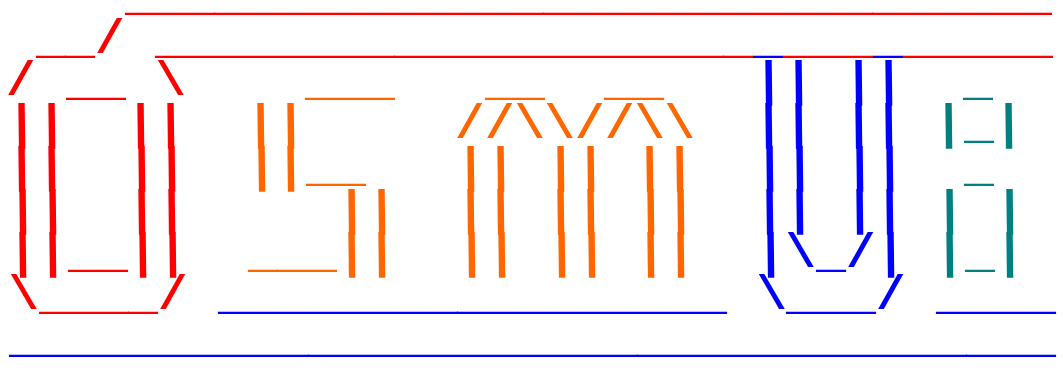
\includegraphics[width=15cm]{../projektplan/Logo_Osmui.png} \\ 
Handbuch von OsmUi}

\begin{document}
\maketitle
\newpage
\tableofcontents
\newpage

\section{Hinweise}
\subsection{Autoren und Website}
\subsection{Leserkreis}
Dieses Handbuch richtet sich an alle Benutzer von OsmUi und die, die es werden wollen.
\subsection{Unterstützte Plattformen}
OsmUi bestet nur aus Java-Code. Daher läuft es auf allen Java SE kompatiblen Systemen, z.B. Linux oder Windows.


\section{Download und Installation}
\subsection{Download des Programms}
\subsection{Installation und Programmstart}
OsmUi wird als ausführbares JAR Archiv ausgeliefert, welches direkt ausgeführt werden kann. 

\section{Beschreibung des Programms}

\section{Anfangsbildschirm}
Nach dem Start von OsmUi ist immer eine leere Datei zu sehen. Es besteht nun die Möglichkeit entweder eine Datei zu laden/exportieren oder eine neue Pipeline zu erstellen.

\section{Aufbau des Bildschirms}
Den größten Teil des Bildschirms nimmt die Pipelinebox ein. Sie befindet sich rechts im Bild und zeigt die aktuelle Pieline. Unter ihr wird die aktuelle Pipeline als Osmosis-Aufruf angezeigt. Links im Bild ist die Taskbox zu sehen. Sie zeigt alle momentan einfügbaren Tasks an. An ihrer Stelle kann auch die Parameterbox stehe, wenn die Parameter eines Tasks geändert werden. 

\section{Laden und Speichern}
Um Pipelines mit allen Details wie Position von verschobenen Tasks, sowie nicht ausführbare Pipelines speichern zu können, verwendet OsmUi ein eigenes Dateiformat (.smu).
\subsection{Datei laden}
Um eine gespeicherte Pipeline zu laden wählt man \textbf{Datei} $\rightarrow$ \textbf{Laden...}. Es öffnet sich ein Dialogfenster, über das man den Pfad zur gewünschten Datei wählen kann. Der Ladevorgang muss nun nur noch bestätigt werden. Es können nur .smu-Dateien geladen werden.
\subsection{Pipeline speichern}
Um die aktuelle Pipeline zu speichern wählt man \textbf{Datei} $\rightarrow$ \textbf{Speichern}. Wenn die Pipeline schon einmal gespeichert wurde, wird die Speicherdatei nur überschrieben. Ansonsten öffnet sich das Speichern-unter-Menü. 
\subsection{Pipeline speichern unter}
Um die aktuelle Pipeline zu speichern wählt man \textbf{Datei} $\rightarrow$ \textbf{Speichern unter...}. Es öffnet sich ein Dialogfenster, in dem man den Speicherort und den gewünschten Namen angeben kann. Nach dem Bestätigen wird eine Speicherdatei neu erstellt. 

\section{Import und Export}
Um mit anderen Osmosis Oberflächen und bereits gesammelten Osmosis Aufrufen kompatibel zu bleiben, bietet OsmUi verschiedene Im- und Export Funktionen an. Dabei können nur konsistente Pipelines exportiert werden.
\subsection{Pipeline importieren aus Zwischenablage}
Beim Importieren aus der Zwischenablage wird der Osmosis Aufruf direkt aus der
Zwischenablage gelesen und die Pipeline geladen. Dazu wählt man \textbf{Datei} $\rightarrow$ \textbf{Importieren aus Zwischenablage}.
\subsection{Pipeline importieren aus Datei}
Hierbei liest OsmUi den Osmosis Aufruf aus einem Aufrufskript. Es werden sowohl .bat
Dateien, als auch .sh Dateien unterstützt. Dazu wählt man \textbf{Datei} $\rightarrow$ \textbf{Importieren aus Datei}.
\subsection{Pipeline exportieren}
OsmUi kann Pipelines als Aufrufskript im .sh Format für alle Posix Konformen Systeme, sowie im .bat Format für Windows exportieren. Der Pfad mit dem Osmosis aufgerufen wird, kann dabei vom Benutzer eingestellt werden. Falls dieser zu einer .jar Datei zeigt wird ''java -jar ” davor gehängt. Dazu wählt man \textbf{Datei} $\rightarrow$ \textbf{Exportieren}.


\section{Pipelinebearbeitung}
\subsection{neue Pipeline erstellen}
Um eine neue Pipeline zu erstellen, wählt man \textbf{Datei} $\rightarrow$ \textbf{Neu}. War zuvor eine Pipeline vorhanden, so wird eine neue leere Instanz von OsmUi geöffnet.

\subsection{Task hinzufügen}
\subsubsection{Input-Tasks}
Um einen Task ohne Eingäng hinzuzufügen wählt man in der Taskbox den gewünschten Input-Task aus und bestätigt mit dem Button ''Hinzufügen''
\subsubsection{Tasks mit Eingängen}
Um einen Task hinzuzufügen muss zuerst in der Pipelinebox der Task selektiert werden, an den angehängt werden soll. Dies geschieht durch einen Einfachklick. Nun werden in der Taskbox alle kompatiblen Tasks angezeigt. Von diesen kann einer angehängt werden, in dem man ihn selektiert und dann auf ''Hinzufügen'' klickt
\subsection{Tasks verbinden}
Sollen zwei bereits vorhandene Tasks verbunden werden, so fährt man mit der Maus über den Task, bis dieser grün umrandet wird. Nun macht man einen Linksklick auf den Task und zieht den entstehenden Pfeil auf den anzuhängenden Task.
\subsection{Task entfernen}
Soll ein Task entfernt werden, so muss man ihn selektieren (Einfachklick) und dann die Entfernen-Taste auf der Tastatur drücken. 
\subsection{Taskparameter ändern}
Um die Parameter eines Task zu ändern macht man einen Doppelklick auf den entsprechenden Task. Nun werden links im Parametertab die Parameter angezeigt. Diese können nun geändert werden. Dabei müssen alle Felder ausgefüllt werden. 
\subsection{Verbindung entfernen}
Um die Verbindung zwischen zwei Tasks zu entfernen, muss man sie selektieren (Einfachklick). Dann drückt man die Entfernen-Taste auf der Tastatur. 

\section{Osmosis-Aufruf kopieren}
Der Osmosis-Aufruf kann aus der Kopierleiste kopiert werden, um ihn zum Beispiel in andere Dokumente einzubinden. Dazu muss man ihn markieren und dann Strg+C auf der Tastatur drücken. Der Aufruf kann nun aus der Zwischenablage importiert werden.

\section{Extras}
\subsection{Rückgängig machen}
Soll eine Änderung wieder rückgängig gemacht werden, so wählt man \textbf{Bearbeiten} $\rightarrow$ \textbf{Rückgängig}.
\subsection{Wiederherstellen}
Soll ein rückgängig gemachter Schritt wiederhergestellt werden, so wählt man \textbf{Bearbeiten} $\rightarrow$ \textbf{Wiederherstellen}.

\section{Programm beenden}
Um OsmUi zu beenden wählt man \textbf{Datei} $\rightarrow$ \textbf{Beenden}.

\section{Versionsgeschichte}
\begin{itemize}
\item Version 1.0 - Erstellung des Handbuchs (04.01.11)
\end{itemize}

\end{document}
